%(BEGIN_QUESTION)
% Copyright 2006, Tony R. Kuphaldt, released under the Creative Commons Attribution License (v 1.0)
% This means you may do almost anything with this work of mine, so long as you give me proper credit

Dampvarmere er nesten alltid laget med \textit{motstrømsdesign}, der de to fluidene strømmer i motsatt retning:

$$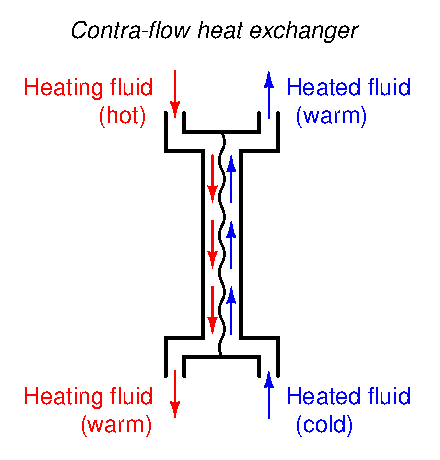
\includegraphics[width=15.5cm]{i00335x01.eps}$$

Dette er helt bevisst. Hvis fluidene i stedet strømmet i samme retning, ville varmeveksleren vært betydelig mindre effektiv:

$$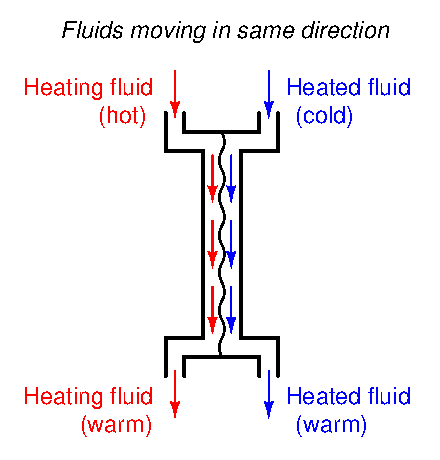
\includegraphics[width=15.5cm]{i00335x02.eps}$$

\vskip 10pt

Forklar hvorfor, gjerne med henvisning til likningen ${dQ \over dt} = {kA {\Delta T} \over l}$.

\underbar{file i00335}
%(END_QUESTION)





%(BEGIN_ANSWER)

I en varmeveksler der begge fluidene går i samme retning, kan det oppvarmede fluidet aldri forlate varmeveksleren med høyere temperatur enn det oppvarmende fluidet har ved utløp. Med motstrømsdesign kan det det.

%(END_ANSWER)





%(BEGIN_NOTES)

Poenget her er at varmeledning gjennom konduksjon (gjennom rørvegger i varmeveksleren) bare skjer når det finnes en temperaturforskjell, i tråd med likningen:

$${dQ \over dt} = {kA {\Delta T} \over l}$$

Hvis det oppvarmede fluidet på en eller annen måte skulle forlate veksleren varmere enn det oppvarmende fluidet gjør, ville varmeflyten nær utløpsenden gått feil vei.

%INDEX% Physics, heat and temperature: heat exchangers

%(END_NOTES)
